% Final Report
% The final reports should be in the style of a short research paper of three pages (about one page text plus plots & figures).
% The format for the report has to be the standard IEEE conference format: https://www.ieee.org/conferences/publishing/templates.html

\documentclass[conference]{IEEEtran}
\usepackage{amsmath,amssymb,amsfonts}
\usepackage{algorithmic}
\usepackage{cite}
\usepackage{bm}
\usepackage{graphicx}
\usepackage{textcomp}
\usepackage{xcolor}
\usepackage[caption=false,font=footnotesize]{subfig}

% \usepackage{subcaption}
% \captionsetup{compatibility=false}


\def\BibTeX{{\rm B\kern-.05em{\sc i\kern-.025em b}\kern-.08emT\kern-.1667em\lower.7ex\hbox{E}\kern-.125emX}}


\begin{document}


\title{Neural Networks for Inverse Kinematics Problems in Robotics}

\author{\IEEEauthorblockN{Franziska Schwaiger}
    \IEEEauthorblockA{\textit{Matriculation number: 03658670}}
    \and
    \IEEEauthorblockN{Thomas Barthel Brunner}
    \IEEEauthorblockA{\textit{Matriculation number: 03675118}}
}

\maketitle

\section*{Introduction}

In our project, we are evaluating the feasibility of using neural networks for inverse kinematics problems in robotics. In this report, we outline the progress made and discuss the results we have obtained.

\section*{Methods}
\subsection*{Robot Simulations}

To train and test our models, we developed simulations of planar robotic arms with revolute joints. As we are interested in testing the limits of our models, we created simulations of arbitraty degrees of freedom (DOFs). In general, the forward kinematics equations of a planar robot arm with link lengths \( l_i \) and \( N \) revolute joints with joint angles \( \theta_i \) can be described as:
\begin{equation}
    x_{TCP} = \sum_{i=1}^{N}{l_i \cos\left( \sum_{j=1}^{i}{\theta_j} \right)}
\end{equation}
\begin{equation}
    y_{TCP} = \sum_{i=1}^{N}{l_i \sin\left( \sum_{j=1}^{i}{\theta_j} \right)}
\end{equation}
\begin{equation}
    \theta_{TCP} = \sum_{i=1}^{N}{\theta_i}
\end{equation}

These equations were modified for fast vectorized numerical computation by the element-wise computation of the sine and cosine of the matrix multiplication of the joint angles vector \( \bm{\theta} = \left[ \theta_1, \theta_2 , ... \right]^\text{T} \) with an upper triangular matrix with ones as elements \( \bm{U} \). The results are then multiplied with the link lengths vector \( \bm{l} = \left[ l_1, l_2, ... \right]^\text{T} \), as shown in Equations \ref{xtcp vectorized} and \ref{ytcp vectorized}.
\begin{equation}
    x_{TCP} = \cos \left( \bm{\theta}\ \bm{U} \right) \bm{l}
    \label{xtcp vectorized}
\end{equation}
\begin{equation}
    y_{TCP} = \sin \left( \bm{\theta}\ \bm{U} \right) \bm{l}
    \label{ytcp vectorized}
\end{equation}

In our current setup, we do not take the angle of the tool center point (TCP) into consideration. Thus, the location of the TCP is defined by its \( x, y \) coordinates. As a result of this, all simulations with more than 2 DOF can up to infinite solutions of the inverse kinematics for a given TCP position. The 2 DOF robot arm can have up to two solutions.

\subsection*{Dataset}

The dataset used for training is composed of one million samples of robot configurations for each DOF. Figure~\ref{fig:datasets} shows an illustration of the datasets. Each configuration was sampled from a normal distribution $ \theta_i \sim \mathcal{N}(\mu=0, \sigma=0.2) $. Thus, the dataset is composed mostly of configurations in which the robot arm is extended. This reflects real-world use cases of robot arms, which have limited workspaces and whose tasks are focused on one section of the workspace. Moreover, limiting the range of the joints improved the performance of the networks, as this avoids the discontinuity in the angles at \( \theta = \pi \).

% TODO add images of datasets

\subsection*{Considering Singularities}

As already mentioned in the previous section, we avoid discontinuities by restricting the configuration space of the robot. Yet we implemented two approaches which consider this discontinuity in the angles at $\theta \in (- \pi , \pi)$ to extend the implemented networks to inverse kinematics problems with general configuration spaces.

The first approach is a non-minimal parameterization of the configuration space as it uses a vector-based representation which was already described in the midterm report to avoid singularities at the boundaries of the joint angles. The drawback of this approach is that the input space is doubled which becomes more and more a problem when increasing the amount of revolute joints of the planar robot.

Therefore, we also considered an alternative approach where we just consider the joint angles resulting in a minimal-reparameterization of the configuration space, again. The discontinuities are now considered in the loss function for the reconstruction error of the of the joint angle space. It ensures that, for example when having a ground truth joint angle $\theta _{gt} = 178^\circ$ and a predicted joint angle $\theta _{pred} = -178^\circ$, the difference between these two angles is only $4^\circ$ instead of $356^\circ$ resulting in a smaller loss.

\subsection*{Network Architectures}

As described in the midterm report, we implemented two network architectures for generating the full posterior distribution of the joint angles: Unlike Variational Autoencoders (VAE), conditional Variational Autoencoders (cVAE) are able to control the data generation process by conditioning the latent space $z$. Considering the application of inverse kinematics,  samples are drawn from $p(z) \sim N(0, 1)$ and the predicted posterior distribution of the joint angles is then generated conditioned on the end-effector position.

Invertible Neural Networks (INN) model a bijective mapping from the joint angles to the end-effector position by stacking invertible blocks together. Here, the dimensionality of the joint angles $x$ is the same as the concatenated output consisting of the latent space $z$ and the end-effector position $y$. The predicted posterior of the joint angles is then generated similar to cVAE by sampling from $p(z) \sim N(0, 1)$ and then running the network backwards conditioned on $y$.

Additionally, INNs share properties with normalizing flows \cite{normalizingFlows2010, normalizingFlows2013} which gradually transform a normal density into the desired data density. They are also bijective and for both normalizing flows and INNs, a tractable Jacobian exists which allows explicit computation of posterior probabilities. As the focus in this work lies on the comparison between cVAE and INN, normalizing flows are not considered anymore.

As stated in \cite{Ardizzone2018}, the INN only needs to be trained on the well-understood forward process and then the inverse process can be obtained for free by just running the network backwards at prediction time. The authors also mention that results can be improved with additional unsupervised backward training. When applying INNs to the inverse kinematics problem, we found that to match the performance of the cVAE, unsupervised brackward training is crucial. This results in two network passes per training step to accumulate the gradients and slows down training a lot. Additionally, when training INNs the parameters need to be adjusted carefully as training can be become unstable.

\subsection*{Hyperparameter Optimization}

For our tests, we trained a network for each robot simulation (DOF). Thus, the sizes and selection of hyperparameters of each network had to match the complexity of the simulation. To compare the performance of the networks across different DOFs in a fair setting, we used Tune \cite{liaw2018tune} to perform a random search of the hyperparameters. To reduce computation time, we trained the models using a subset of the main dataset, which was composed of \( 1e4 \) samples.

% TODO eventually add table with tuned parameters and 
% the range of the parameters!

\subsection*{Implementation}

The previous two model architectures (cVAE and INN) have been implemented in PyTorch and are inspired by existing implementations in  \cite{graviraja2019, freia2020}. We utilized the Google Compute Engine to train our models.

\section*{Experimental Evaluation}

\subsection*{Evaluation protocol}

We extended the degrees of freedoms (DoF) of the robots up to 10 DoF and performed hyperparameter optimization (HPO) for the hyperparameters for $DoF = [6, 8, 10]$ by evaluating $100$ points in the hyperparameters space for each DoF. But now it is important to mention that due to HPO, the number of trainable parameters differs between cVAE and INN. The batch size is kept fixed to $1000$ for both networks.
For the cVAE, we optimized the learning rate, the weight decay, the number of hidden layers for the encoder and decoder and the amount of neurons per layer. For the INN, we optimized the learning rate, the weight decay, the number of coupling layers, the amount of layers per subnet and also the number of neurons per subnet layer.
Both networks have been trained for 60 epochs on a dataset with 1 million samples and a train and test spit of 70 and 30, respectively. For evaluation, we used again the two evaluation metrics which have been described in the midterm report:

1. The average posterior mismatch between the distribution generated by the model and the ground truth estimate obtained via rejection sampling. For generating the posterior, we used 100 samples per ground truth position and averaged over 1000 samples from the dataset.

2. The average re-simulation error as the mean squared distance between the ground truth end-effector position and the re-simulated end-effector position obtained from the predicted joint angles. The re-simulation error was averaged over the whole test dataset.

\subsection*{Results}

%%%%%%%%%%%%%%%%%%%%%%
% TABLES
%%%%%%%%%%%%%%%%%%%%%%
\begin{table*}[h]
\centering
\begin{tabular}{|c|c|c|c|c|c|}
\hline
 DOF & learning rate & weight decay & \# hidden layers & \# neurons & \# trainable parameters\\
 \hline
 6  & ... & ...& ... & ... & ...\\
 10  & ... & ... & ... & ... & ...\\
 15  & ... & ... & ... & ... & ...\\
 \hline
\end{tabular}
\vspace{5pt}
\caption{\label{tab:results:cvae}  Hyperparameters for cvae which has been trained on a planar robot with $N$ DOF with $N=[4, 6, 10, 15]$.}
\end{table*}

\begin{table*}[h]
\centering
\begin{tabular}{|c|c|c|c|c|c|c|}
\hline
 DOF & learning rate & weight decay & \# coupling layers & \# subnet layers & \# neurons per subnet layer &  \# trainable parameters\\
 \hline
 6  & ... & ...& ... & ... & ... & ...\\
 10  & ... & ... & ... & ... & ... & ...\\
 15  & ... & ... & ... & ... & ... & ...\\
 \hline
\end{tabular}
\vspace{5pt}
\caption{\label{tab:results:inn}  Hyperparameters for inn which has been trained on a planar robot with $N$ DOF with $N=[4, 6, 10, 15]$.}
\end{table*}

The hyperparameters for the cVAE and INN chosen by HPO are depicted in Table \ref{tab:results:cvae} and \ref{tab:results:inn}, respectively. Because of HPO, the number of parameters per robot is not approximately equal, anymore. As it can be seen in the tables, the best architectures are not the architectures with the most numbers of trainable parameters. This also shows that the hyperparameters search space is sufficient. 

For both networks, the mismatch of the posterior distribution and the re-simulation error is plotted over the number of parameters in Fig. \ref{fig:plot:posterior} and \ref{fig:plot:resim}, respectively. Each plotted point is labelled with the corresponding robot of different DoF. As it can be seen, when increasing the number of degrees of freedom, the number of parameters does not have to be increased, as well. This is also a result of the HPO. 
The mismatch of the predicted posterior (see Fig. \ref{fig:plot:posterior}) with the ground truth posterior obtained from rejection sampling is less for the INN as for the cVAE. But in contrast to that, the cVAE performs consistently better on the re-simulation error as the INN (see Fig. \ref{fig:plot:resim}).

%%%%%%%%%%%%%%%%%%%%%%
% RESULTS, FIGURES
%%%%%%%%%%%%%%%%%%%%%%
\begin{figure}[!ht]
\centering
	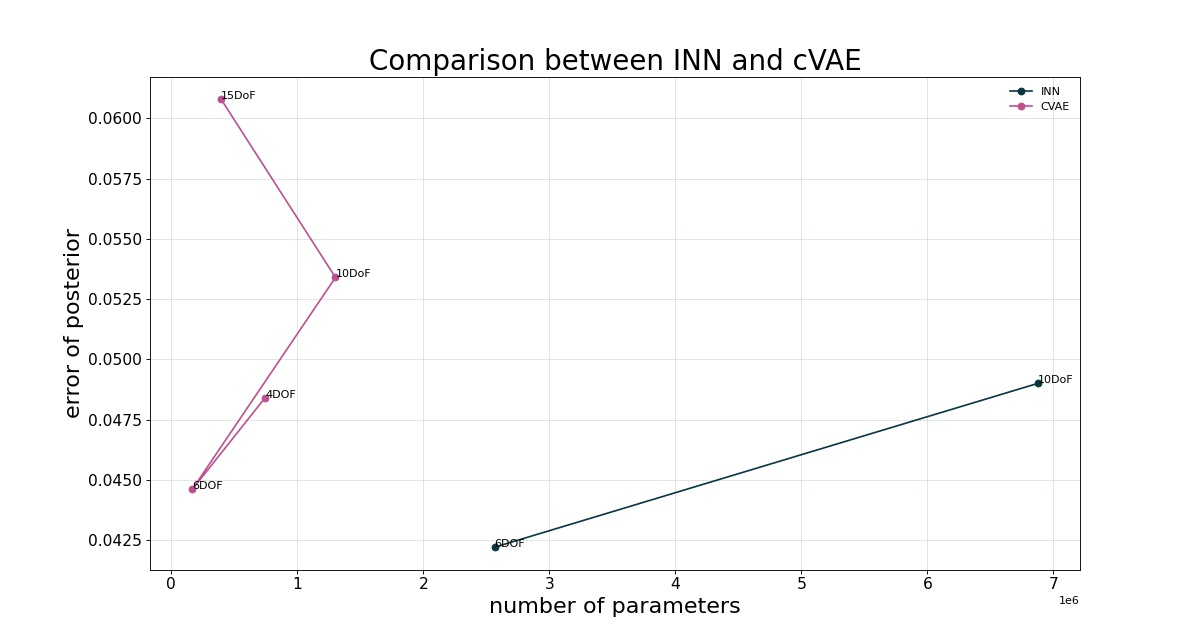
\includegraphics[width=\linewidth]{figures/comparison_e_posterior_alternative.jpg}
    \caption{\label{fig:plot:posterior} Results. Mismatch of posterior. Needs to be completed.}
\end{figure}

\begin{figure}[!ht]
\centering
	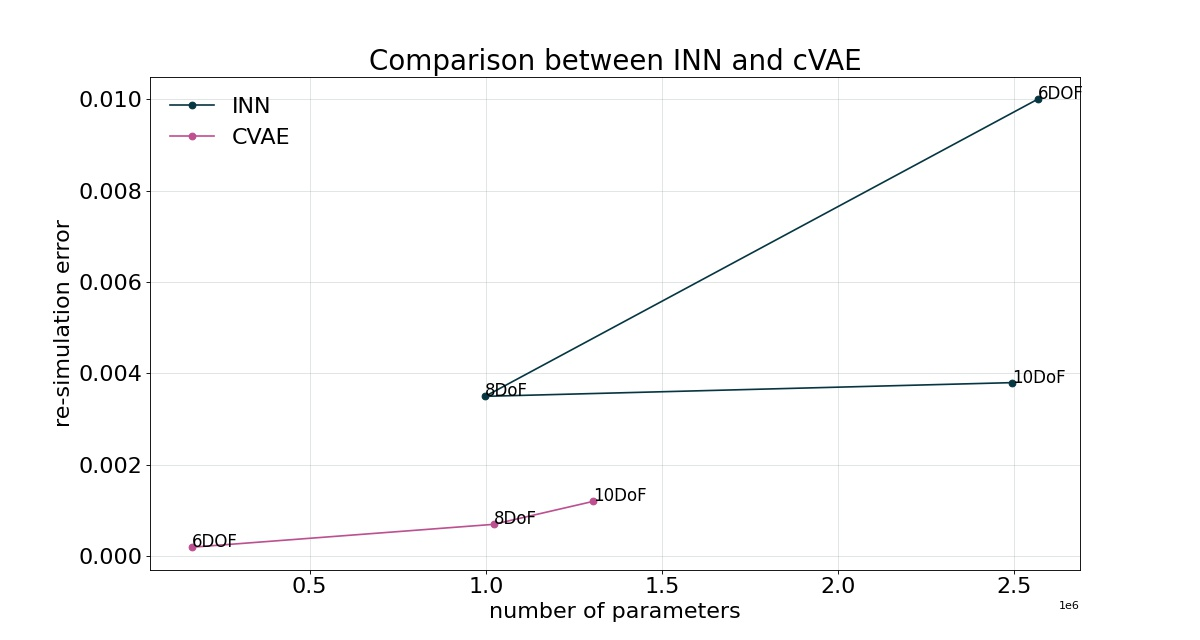
\includegraphics[width=\linewidth]{figures/comparison_e_resim_alternative.jpg}
    \caption{\label{fig:plot:resim} Results. Mismatch of re-simulation error. Needs to be completed.}
\end{figure}

In Fig. \ref{fig:q_quantile:cVAE:6DOF} and \ref{fig:q_quantile:INN:6DOF}, the area of the convex hull of the $97\%$ percentile of $1000$ re-simulated end-effector positions (green dots) with a ground truth at $(x, y) = [3.47, 0.19]$ (red dot) is visualized for the cVAE and INN, respectively.  As it can be seen, the re-simulated points of the INN span a larger convex hull with an area of $0.85$ around the ground truth position than the re-simulated points of the cVAE with an area of $0.15$. This behaviour is also reflected in the chart of the re-simualtion error (see Fig. \ref{fig:plot:resim}) as described previously. But despite of having a larger re-simulation error, the INN recovers the full posterior distribution of the joint angles much better than the cVAE, as it can be seen in Fig. \ref{fig:posterior:6dof}. 

%%%%%%%%%%%%%%%%%%%%%%
% FIGURES, CONVEX HULL
%%%%%%%%%%%%%%%%%%%%%%
\begin{figure*}[tbh]
\centering
	\subfloat[cVAE]{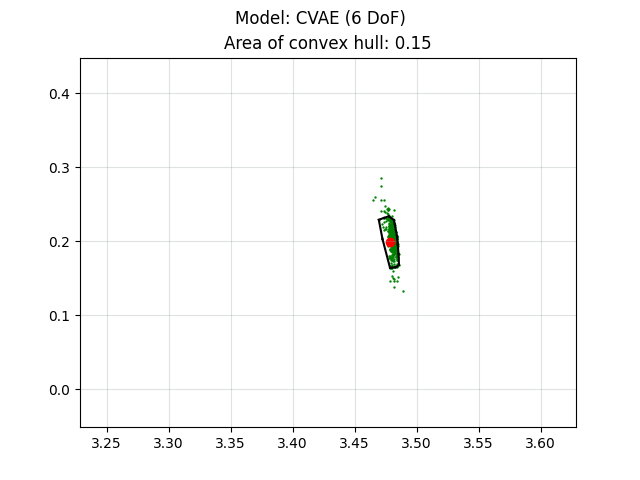
\includegraphics[width=0.47\linewidth]{figures/q_quantile_prediction_CVAE_6DOF.png}
    \label{fig:q_quantile:cVAE:6DOF}}
    %
    \subfloat[INN]{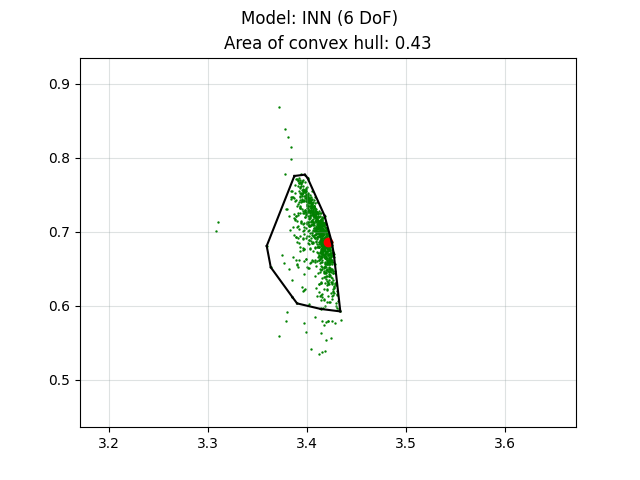
\includegraphics[width=0.47\linewidth]{figures/q_quantile_prediction_INN_6DOF.png}
        \label{fig:q_quantile:INN:6DOF}}

    \caption{\label{fig:q_quantile:cVAE:6dof} Area of the convex hull of the 0.97 percentile of the re-simulated end-effector coordinates with the ground truth end-effector position at $(x, y) = [3.47, 0.19]$ and $1000$ samples. Number of DoF: 6.}
\end{figure*}
%%%%%%%%%%%%%%%%%%%%%%
% FIGURES, POSTERIOR
%%%%%%%%%%%%%%%%%%%%%%
\begin{figure*}[tbh]
\centering
	\subfloat[Rejection Sampling]{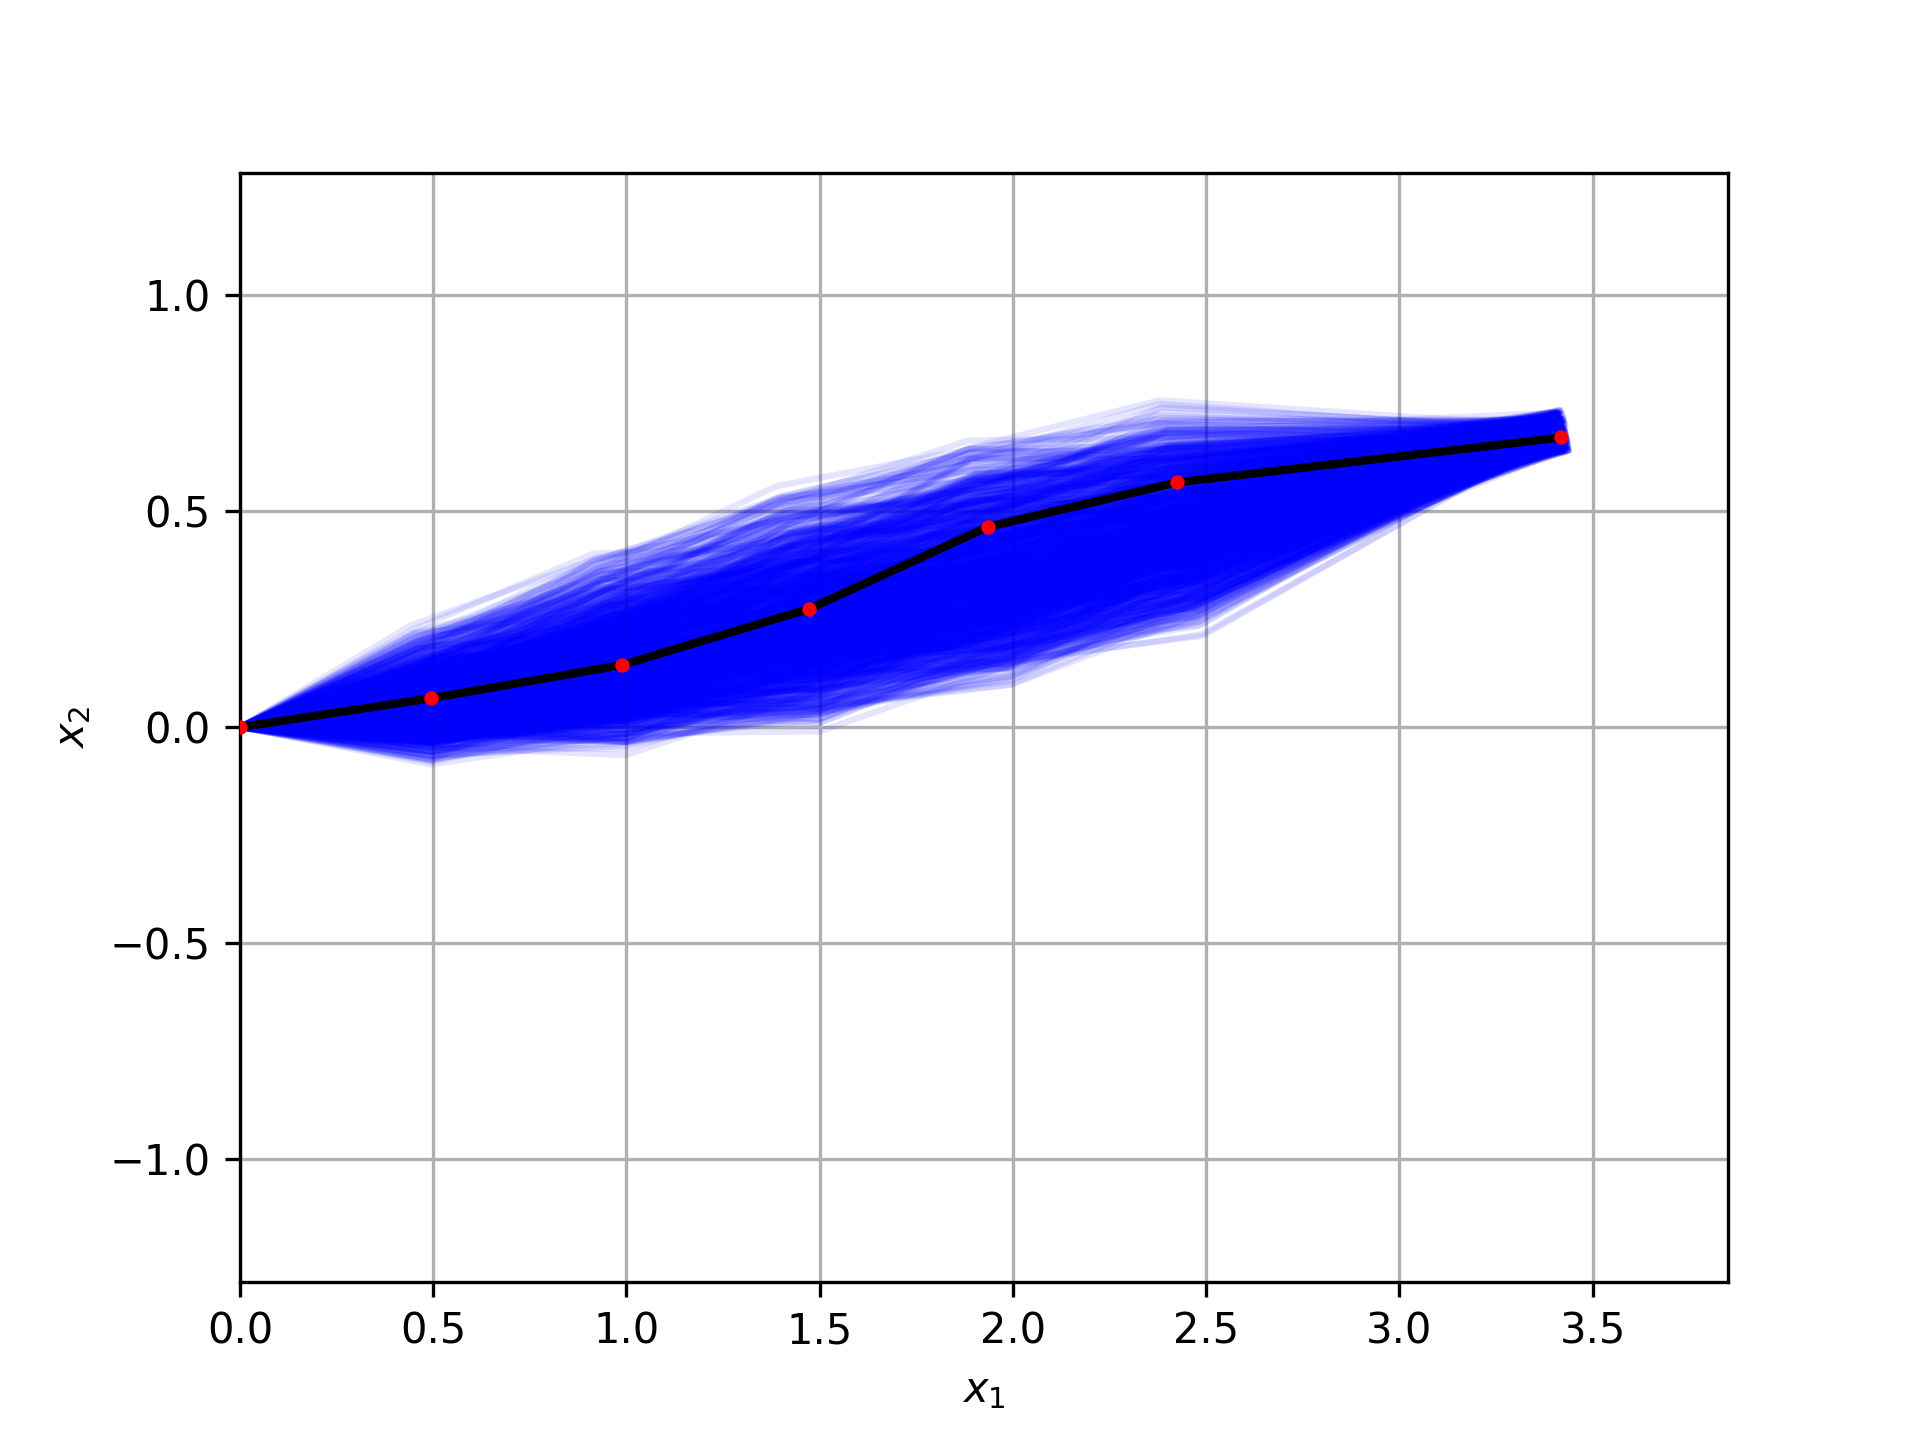
\includegraphics[width=0.32\linewidth]{figures/rejection_sampling_INN_6DOF.png}
    \label{fig:rejection_sampling:6DOF}}
    %
    \subfloat[cVAE]{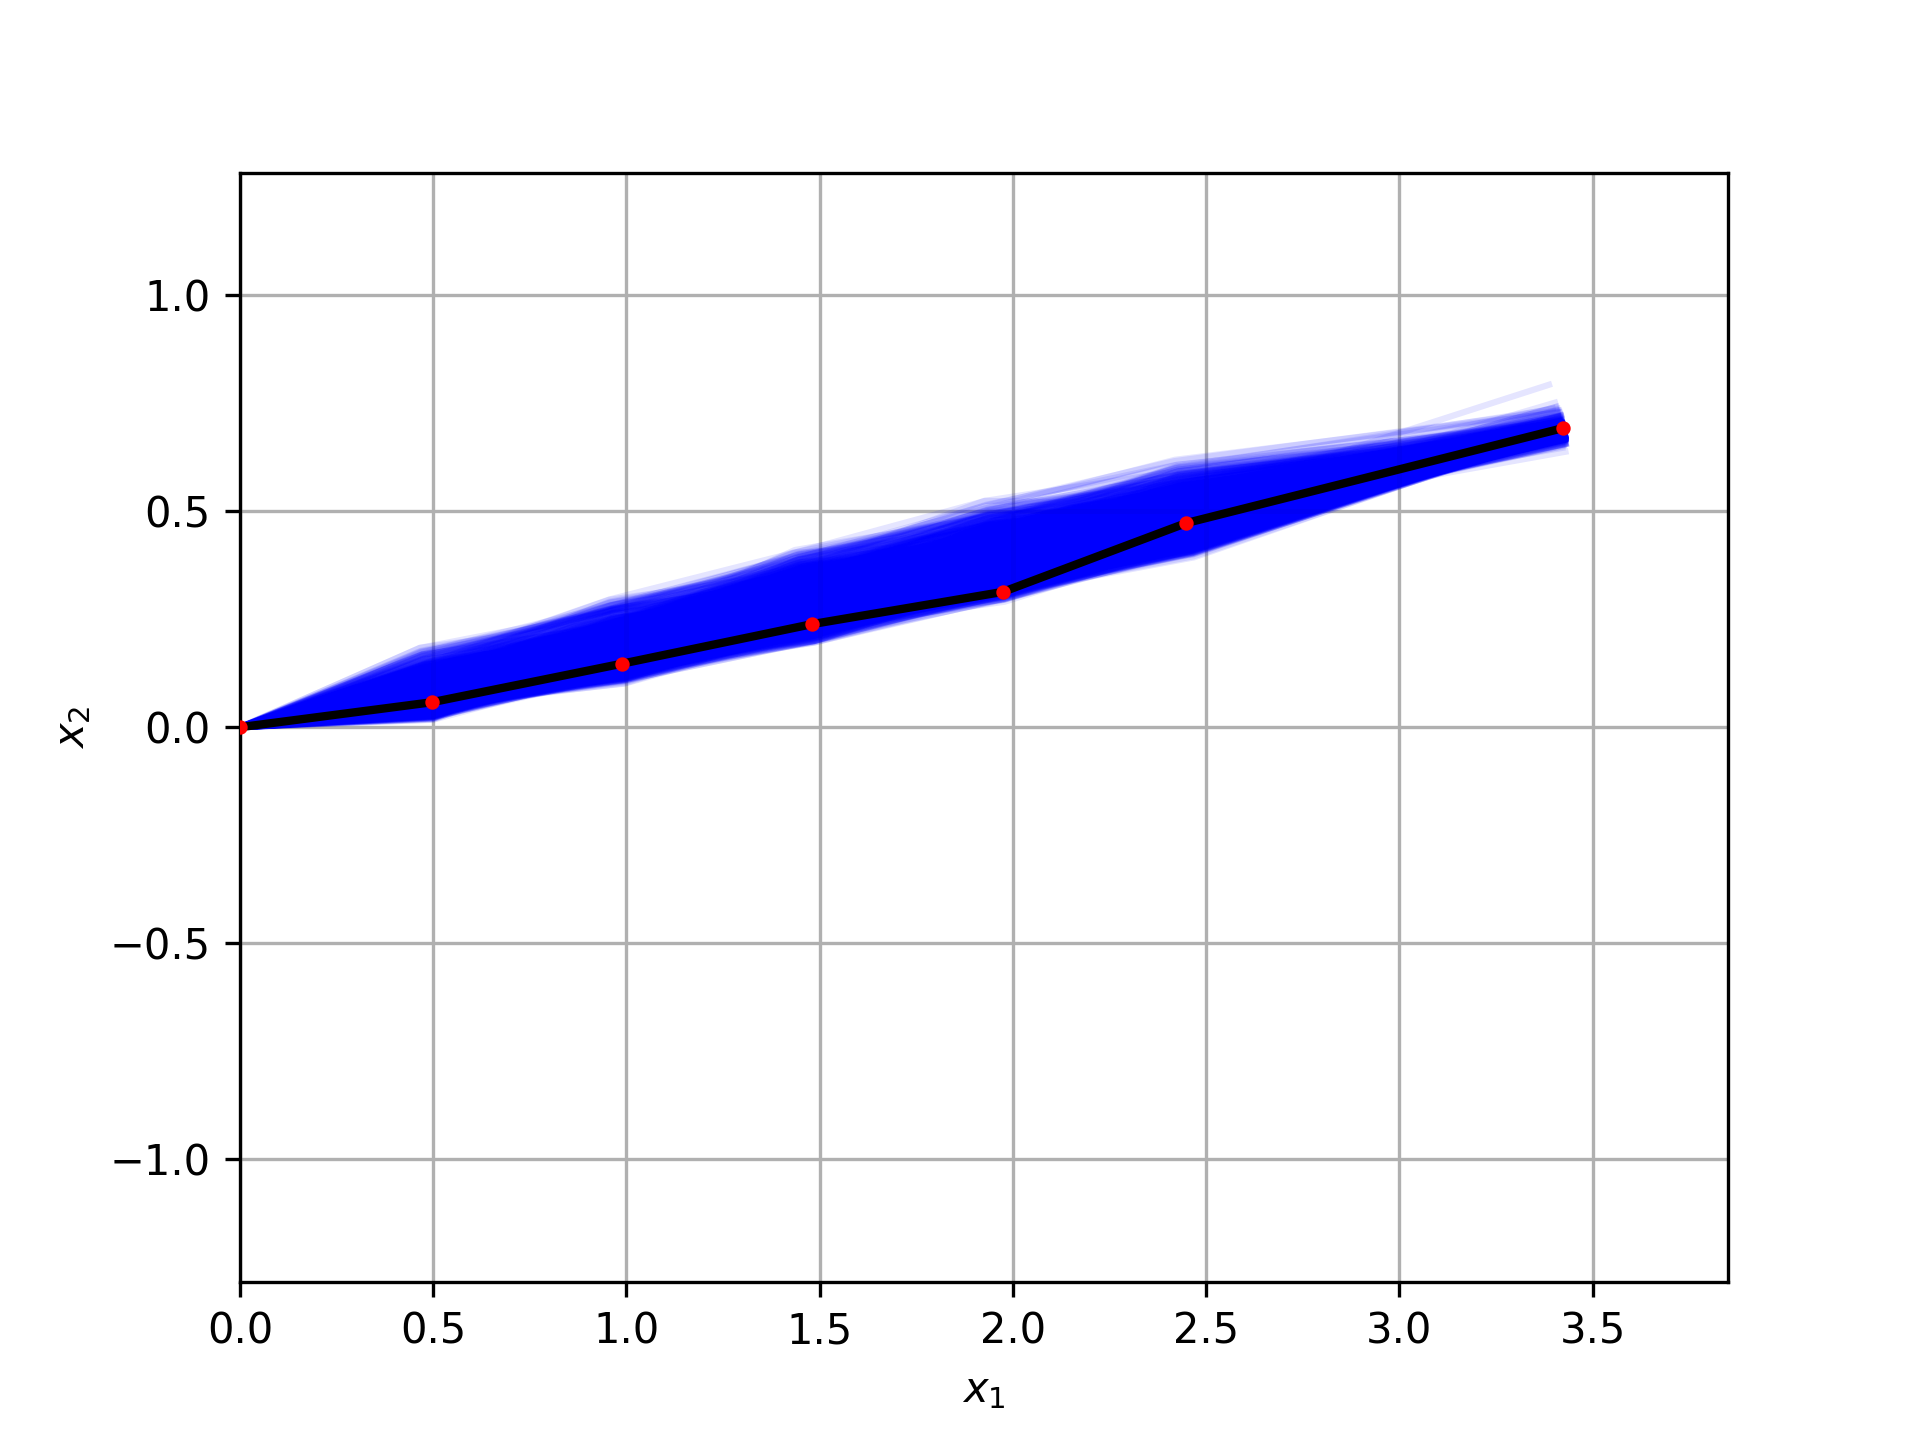
\includegraphics[width=0.32\linewidth]{figures/predicted_posterior_CVAE_6DOF.png}
        \label{fig:cVAE:6DOF}}
    %
    \subfloat[INN]{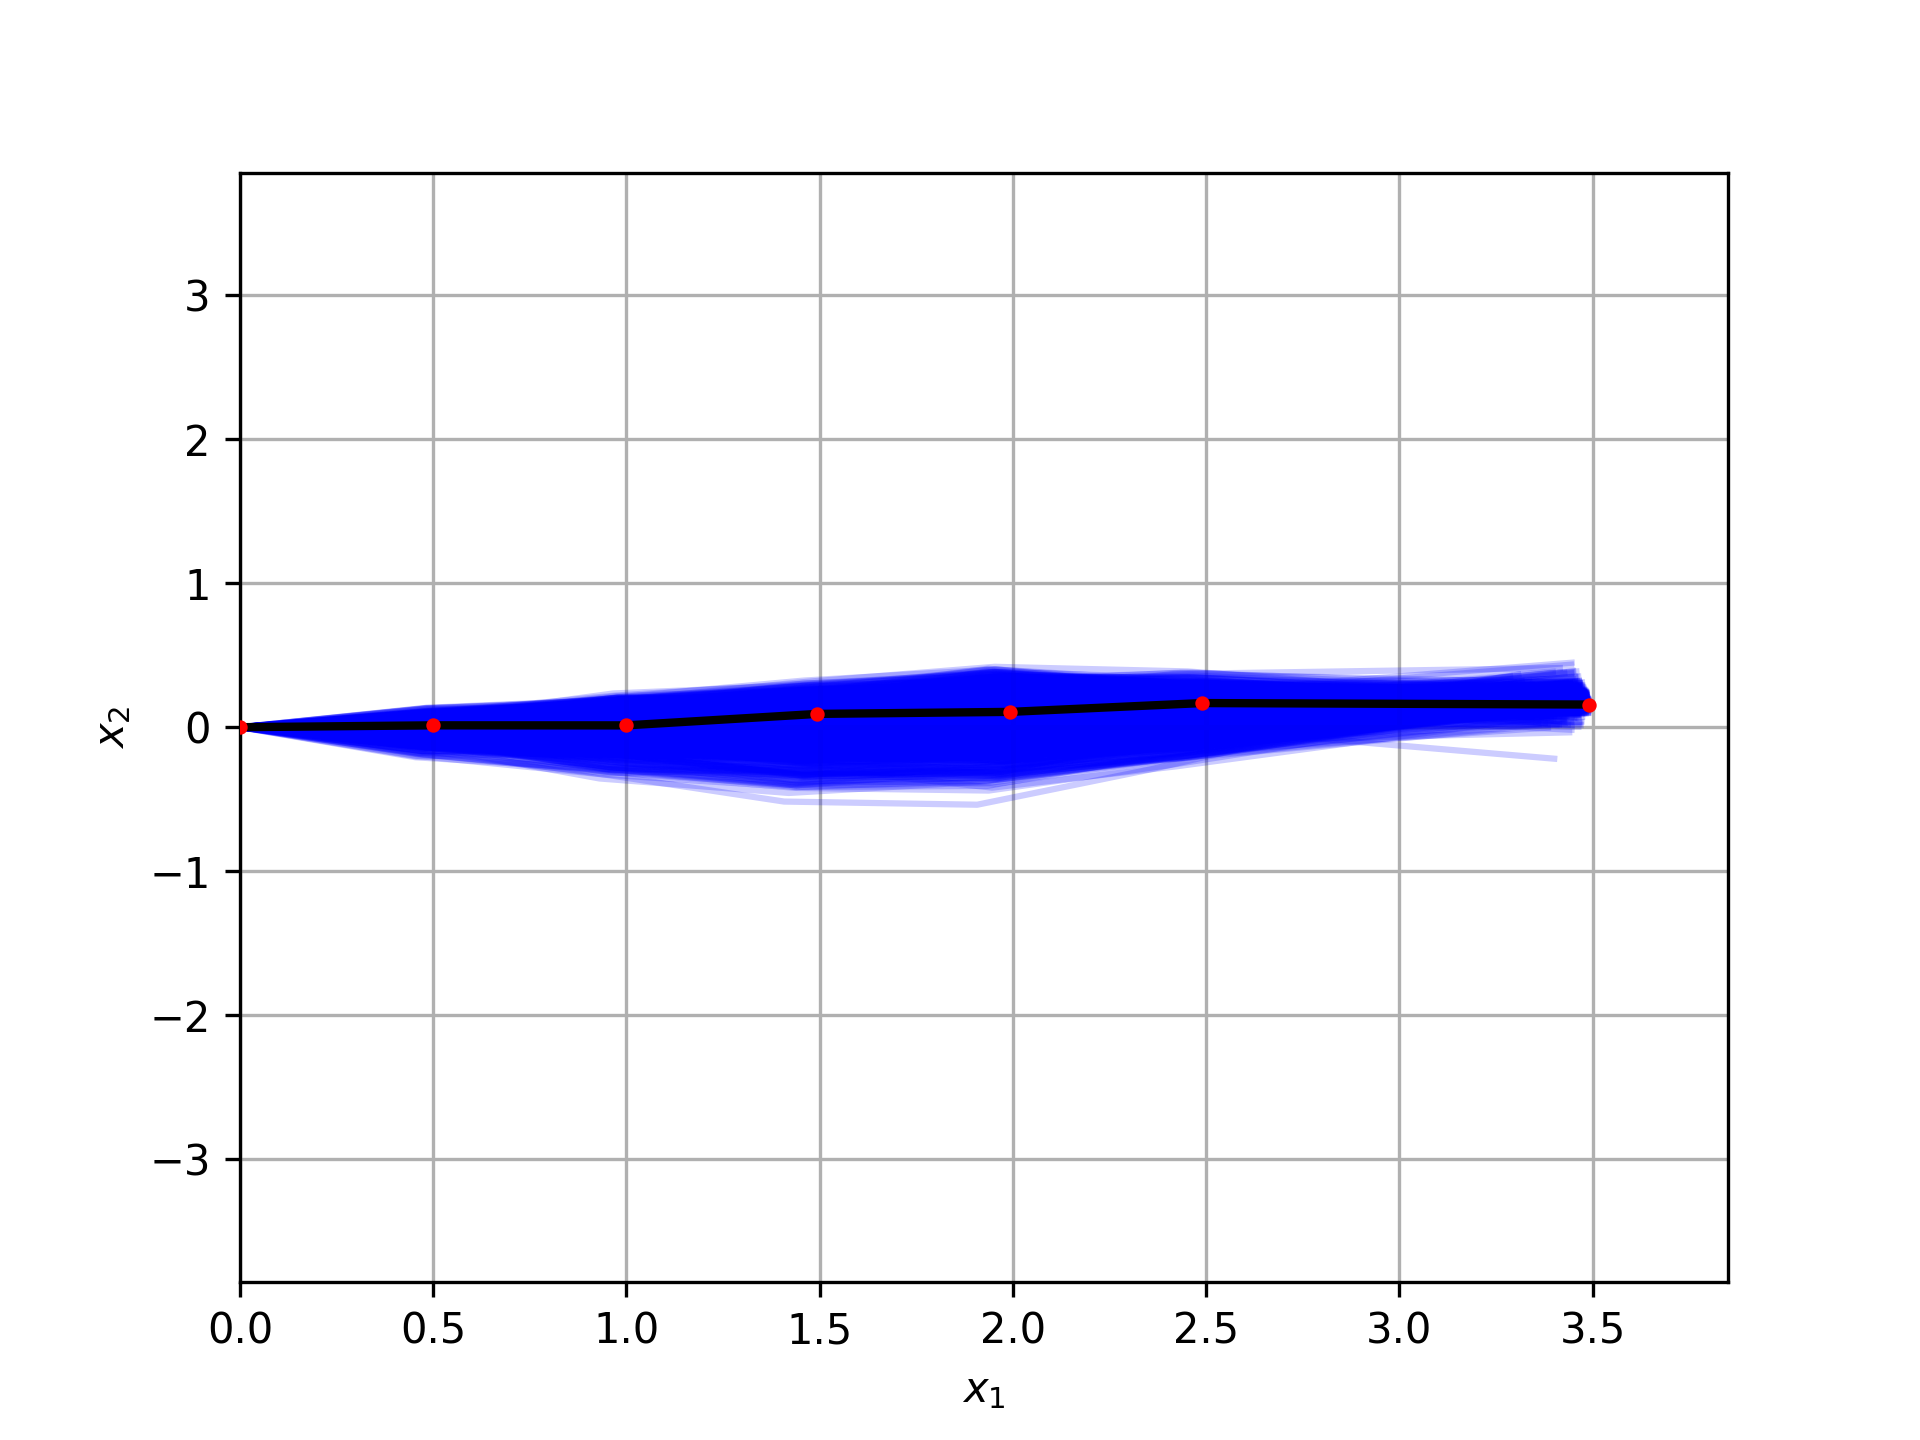
\includegraphics[width=0.32\linewidth]{figures/predicted_posterior_INN_6DOF.png}
        \label{fig:INN:6DOF}}

    \caption{\label{fig:posterior:6dof} Arm configuration of a planar manipulator with $6$ revolute joints and end-effector position at $(x, y) = [3.47, 0.19]$. 100 samples are drawn from each model's predicted posterior $\tilde{p}(x | y_{gt})$, one random sample configuration is highlighted. $e_{posterior} = 0.032$ for the cVAE and $e_{posterior} = 0.018$ for the INN.}
\end{figure*}

\section*{Conclusion}

In this work, we evaluated through simulation experiments the feasability of using neural network architectures to fully recover the posterior distribution of the hidden parameter space in the context of inverse kinematics problems in robotics. For this, we studied invertible neural networks and compared them to conditional Variational Autoencoders using as a baseline. At first, we constructed simple planar robots with up to 4 revolute joints and then extended the simulations with more complex planar robots with up to 15 revolute joints. To find the best set of hyper parameters we performed Bayesian optimization.

Using evaluation metrics defined in previous research, given the end-effector position we found that cVAEs are better in predicting the values of the joint angles which, when applied to forward kinematics again, result in being closer to the ground truth end-effector position. In contrast, experiments show that INNs better recover the full posterior distribution over the joint angle space. 

Unlike stated in previous research, we had to perform an additional unsupervised backward training to match the performance of the cVAE resulting in slowing down the training a lot. Also, INNs tend to be more unstable in the training process as cVAEs. Despite this, INNs are an interesting and powerful tool in not only recovering the full posterior parameters distribution but also being able to explicitly compute the posterior probability by using tractably Jacobians.

\nocite{*}
\bibliographystyle{IEEEtran}
\bibliography{IEEEabrv,final_report}

\end{document}
